\documentclass[
  unicode,a4paper,11pt,aspectratio=169,
  xcolor = {dvipsnames,svgnames},
  hyperref ={colorlinks=true,citecolor=Navy,linkcolor=NavyBlue,urlcolor=purple},
  ja=standard,lualatex
]{beamer}
\renewcommand{\baselinestretch}{1.4}

% ---fonts---
\usefonttheme{serif}
\mathversion{bold}
\usepackage{luatexja-fontspec}
\setmainfont{TeX Gyre Termes}
\setmainjfont{Noto Sans JP}
\setmathrm{Latin Modern Roman}
% \setmainjfont{IPAexGothic}

% ---refer `texdoc xcolor' at the command line---

% ---Display \subsubsection at the Index
% \setcounter{tocdepth}{3}

% ---Setting about the geometry of the document----
% \usepackage{a4wide}
% \pagestyle{empty}

% ---Physics and Math Packages---
\usepackage{amssymb,amsfonts,amsthm,mathtools}
\usepackage{physics,braket,bm}

% ---underline---
\usepackage[normalem]{ulem}

% ---cancel---
\usepackage{cancel}

% --- surround the texts or equations
\usepackage{fancybox,ascmac}

% ---settings of theorem environment---
% \usepackage{amsthm}
% \theoremstyle{definition}

% ---settings of proof environment---
% \renewcommand{\proofname}{\textbf{証明}}
% \renewcommand{\qedsymbol}{$\blacksquare$}

% ---Insert the figure (If insert the `draft' at the option, the process becomes faster.)---
\usepackage{graphicx}
% \usepackage{subcaption}

% ----Add a link to a text---
\usepackage{url,hyperref}
\usepackage{xcolor}

% ---Tikz---
\usepackage{tikz,pgf,pgfplots,circuitikz}
\pgfplotsset{compat=1.15}
\usetikzlibrary{intersections,arrows.meta,angles,calc,3d,decorations.pathmorphing,positioning}

% ---Add the section number to the equation, figure, and table number---
\makeatletter
   \renewcommand{\theequation}{\thesection.\arabic{equation}}
   \@addtoreset{equation}{section}
   
   \renewcommand{\thefigure}{\thesection.\arabic{figure}}
   \@addtoreset{figure}{section}
   
   \renewcommand{\thetable}{\thesection.\arabic{table}}
   \@addtoreset{table}{section}
\makeatother

% ---enumerate---
% \renewcommand{\labelenumi}{$\arabic{enumi}.$}
% \renewcommand{\labelenumii}{$(\arabic{enumii})$}

% ---beamer settings---
\usefonttheme{professionalfonts}
\usecolortheme{seahorse}
\setbeamercolor{structure}{fg=white}
\setbeamercolor{local structure}{fg=red}
\setbeamertemplate{itemize item}[ball]
\setbeamertemplate{enumerate item}[circle]
\setbeamercolor{bibliography entry author}{fg=black}
\setbeamercolor{bibliography item}{fg=black}
\setbeamercolor{alerted text}{fg=RoyalBlue}
\setbeamertemplate{frametitle continuation}{}
\setbeamertemplate{footline}[frame number]
\setbeamertemplate{navigation symbols}{} 

% ---tcolorbox---
\usepackage{tcolorbox}
\tcbuselibrary{raster,skins,theorems}
\newtcolorbox{bluebox}[2][]{enhanced,
colframe=RoyalBlue!40!white,
colback=RoyalBlue!10!white,
coltitle=black,
drop fuzzy shadow, title={#2}
,#1}
\newtcolorbox{redbox}[2][]{enhanced,
colframe=DarkRed!40!white,
colback=DarkRed!10!white,
coltitle=black,
drop fuzzy shadow, title={#2}
,#1}

% ---Ignore the Warnings---
\usepackage{silence}
\WarningFilter{latexfont}{Some font shapes}
\WarningFilter{latexfont}{Font shape}
\ExplSyntaxOn
\msg_redirect_name:nnn{hooks}{generic-deprecated}{none}
\ExplSyntaxOff

% \usepackage{newtxmath}

% ---citation---
% \usepackage{usebib}
% \newbibfield{author} 
% \newbibfield{year} 
% \newbibfield{journal} 
% \newbibfield{doi} 
% \bibinput{ref}

% \makeatletter
% \newcommand*{\journal}{\begingroup\@makeother\#\@mylink}
% \newcommand*{\@mylink}[1]{\href{http://dx.doi.org/\usebibentry{#1}{doi}}{\usebibentry{#1}{journal}}\endgroup} 
% \makeatother

% \newcommand*{\citefone}[2]{
%   \begin{tikzpicture}[remember picture, overlay]
%     \node[anchor=north east, align=left] at ($(current page.north east)-(0,0.0)$){
%     {\tiny
%       \cite{#1}
%       #2,
%       \journal{#1}
%       (\usebibentry{#1}{year}).
%     }
%     };
%   \end{tikzpicture}
% }

% \newcommand*{\citeftwo}[4]{
%   \begin{tikzpicture}[remember picture, overlay]
%     \node[anchor=north east, align=left] at ($(current page.north east)-(0,0.0)$){
%     {\tiny
%       \cite{#1}
%       #2,
%       \journal{#1}
%       (\usebibentry{#1}{year}).
%     }
%     \\[-2.4ex]
%     {\tiny
%       \cite{#3}
%       #4,
%       \journal{#3}
%       (\usebibentry{#3}{year}).
%     }
%     };
%   \end{tikzpicture}
% }

% \newcommand*{\citefthree}[6]{
%   \begin{tikzpicture}[remember picture, overlay]
%     \node[anchor=north east, align=left] at ($(current page.north east)-(0,0.0)$){
%     {\tiny
%       \cite{#1}
%       #2,
%       \journal{#1}
%       (\usebibentry{#1}{year}).
%     }
%     \\[-2.4ex]
%     {\tiny
%       \cite{#3}
%       #4,
%       \journal{#3}
%       (\usebibentry{#3}{year}).
%     }
%     \\[-2.4ex]
%     {\tiny
%       \cite{#5}
%       #6,
%       \journal{#5}
%       (\usebibentry{#5}{year}).
%     }
%     };
%   \end{tikzpicture}
% }

% \newcommand*{\citefonev}[3]{
%   \begin{tikzpicture}[remember picture, overlay]
%     \node[anchor=north east, align=left, text width=#3cm] at ($(current page.north east)-(0,0.0)$){
%     {{\fontsize{5pt}{0pt}\selectfont
%       \cite{#1}
%       #2,
%       \journal{#1}
%       (\usebibentry{#1}{year}).\par}
%     }
%     };
%   \end{tikzpicture}
% }

% \newcommand*{\citeftwov}[5]{
%   \begin{tikzpicture}[remember picture, overlay]
%     \node[anchor=north east, align=left, text width=#5cm] at ($(current page.north east)-(0,0.0)$){
%     {{\fontsize{5pt}{0pt}\selectfont
%       \cite{#1}
%       #2,
%       \journal{#1}
%       (\usebibentry{#1}{year}).\par}

%       {\fontsize{5pt}{0pt}\selectfont
%       \cite{#3}
%       #4,
%       \journal{#3}
%       (\usebibentry{#3}{year}).\par}
%     }
%     };
%   \end{tikzpicture}
% }

% \newcommand*{\citefthreev}[7]{
%   \begin{tikzpicture}[remember picture, overlay]
%     \node[anchor=north east, align=left, text width=#7cm] at ($(current page.north east)-(0,0.0)$){
%     {{\fontsize{5pt}{0pt}\selectfont
%     \cite{#1}
%     #2,
%     \journal{#1}
%     (\usebibentry{#1}{year}).\par}

%     {\fontsize{5pt}{0pt}\selectfont
%     \cite{#3}
%     #4,
%     \journal{#3}
%     (\usebibentry{#3}{year}).\par}

%     {\fontsize{5pt}{0pt}\selectfont
%     \cite{#5}
%     #6,
%     \journal{#5}
%     (\usebibentry{#5}{year}).\par}
%     }
%     };
%   \end{tikzpicture}
% }


% ---Title---
\title{
  卒業研究
  \texorpdfstring{\\}{}
  \texorpdfstring{\vspace*{5pt}}{}
  {\LARGE
    磁化トーラス上にコンパクト化した
    \\
    超対称模型におけるモジュライ固定
  }
}
\author{
  安倍研究室 \ B4
  \texorpdfstring{\\}{}
  \texorpdfstring{\vspace*{3pt}}{}
  宮根 一樹
}
\date{2024年3月1日(金)}


\begin{document}

\begin{frame}
  \titlepage
\end{frame}


\section{イントロダクション}

\begin{frame}
  \huge \secname
\end{frame}

\begin{frame}
  世の中の物質は細かく見ていくことが可能。

  実験的には「素粒子」が今のところ最小の構成要素。

  \begin{center}
    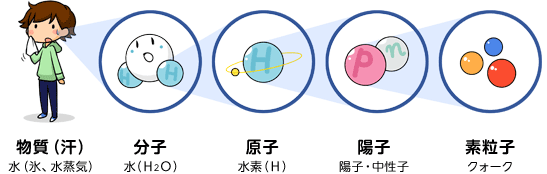
\includegraphics[width=0.8\textwidth]{fig/ILCproject.png}       

    \vspace*{-5pt}
    { \small
      \hspace*{6cm}
      [\href{https://aaa-sentan.org/ILC/about_physics/anatomy01.html}{ILC PROJECT}]
    }   
  \end{center}

\end{frame}

\begin{frame}
  
  \begin{center}

    実験で観測されているのはこの17個の素粒子。
  
    (2012年にヒッグス粒子が発見)

    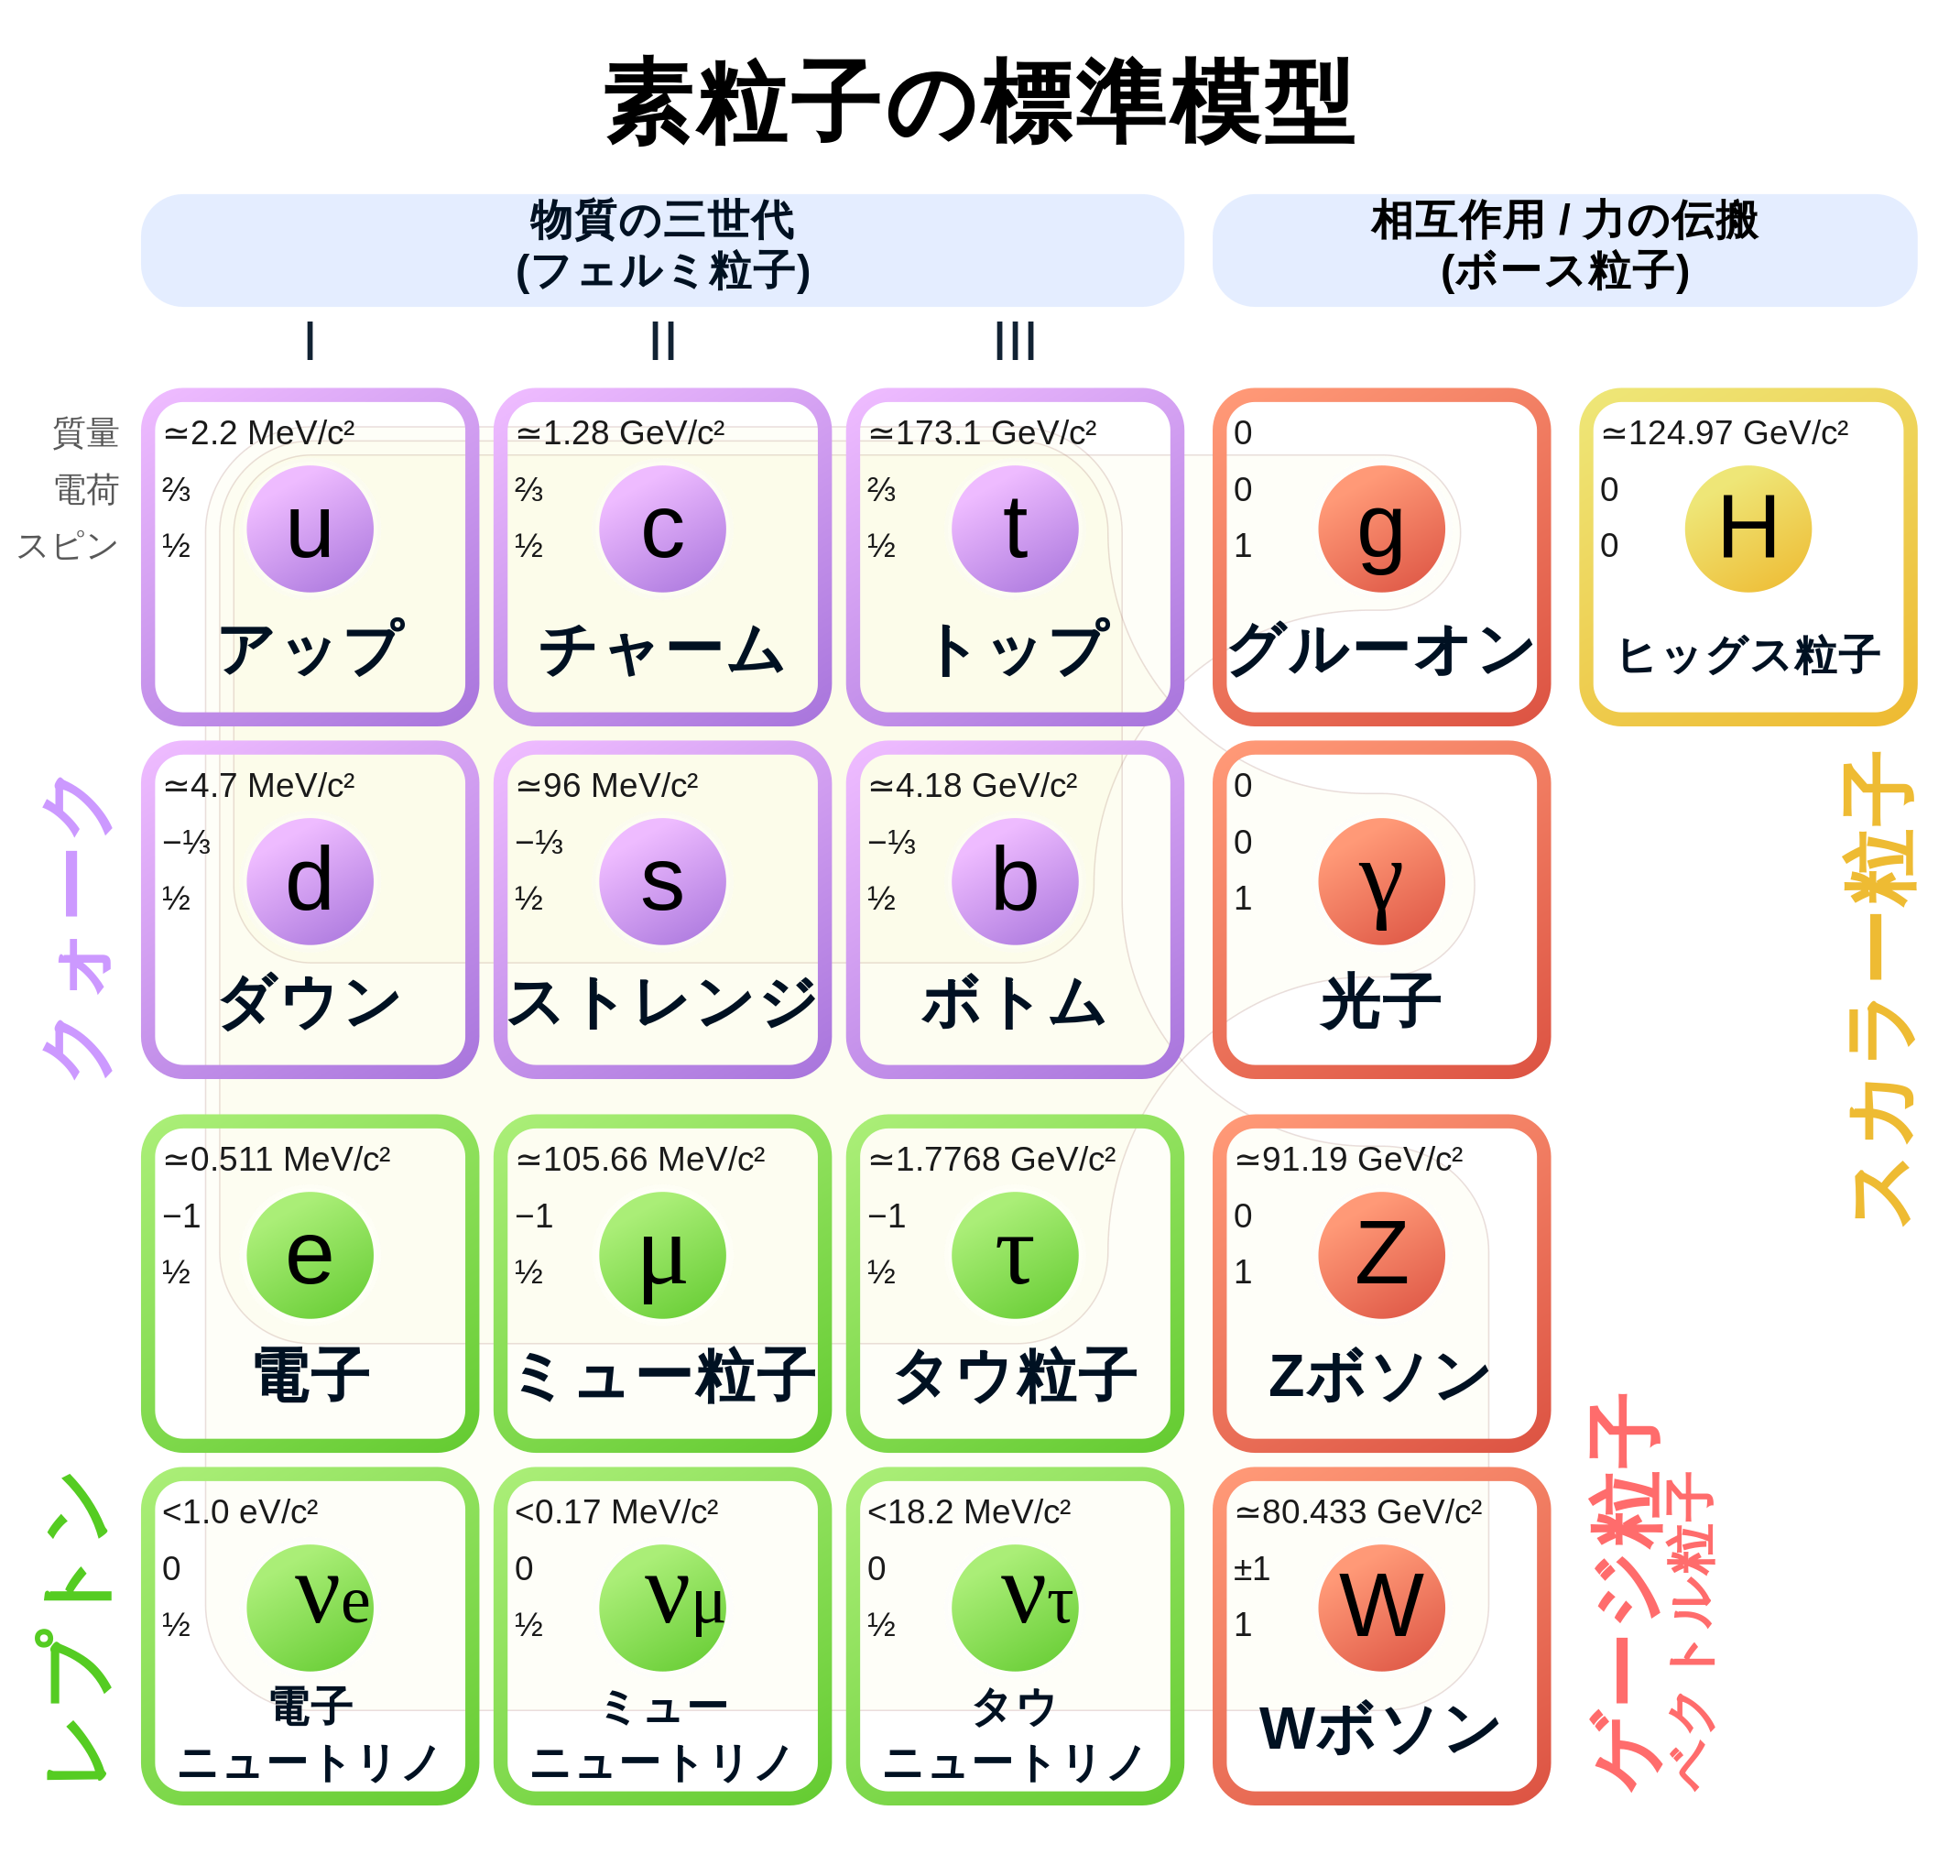
\includegraphics[width=0.4\textwidth]{fig/SM.png}  

    \vspace*{-15pt}
    { \small
      \hspace*{4cm}
      [\href{https://ja.wikipedia.org/wiki/標準模型}{Wikipedia}]
    }
  \end{center}

\end{frame}

\begin{frame}

  この標準模型には、まだ未解決な問題が多数ある。
  
  そもそもどうしてこのような構造をしているのか?

  \begin{itemize}
    \item 
    \textcolor{DarkGreen}{なぜ、}\textcolor{DarkBlue}{物質は3世代存在するのか。}
    \item 
    \textcolor{DarkGreen}{なぜ、}\textcolor{DarkRed}{世代が上がるごとに質量が大きく変わるのか。}
  \end{itemize}

  \only<1>{
    \begin{center}
      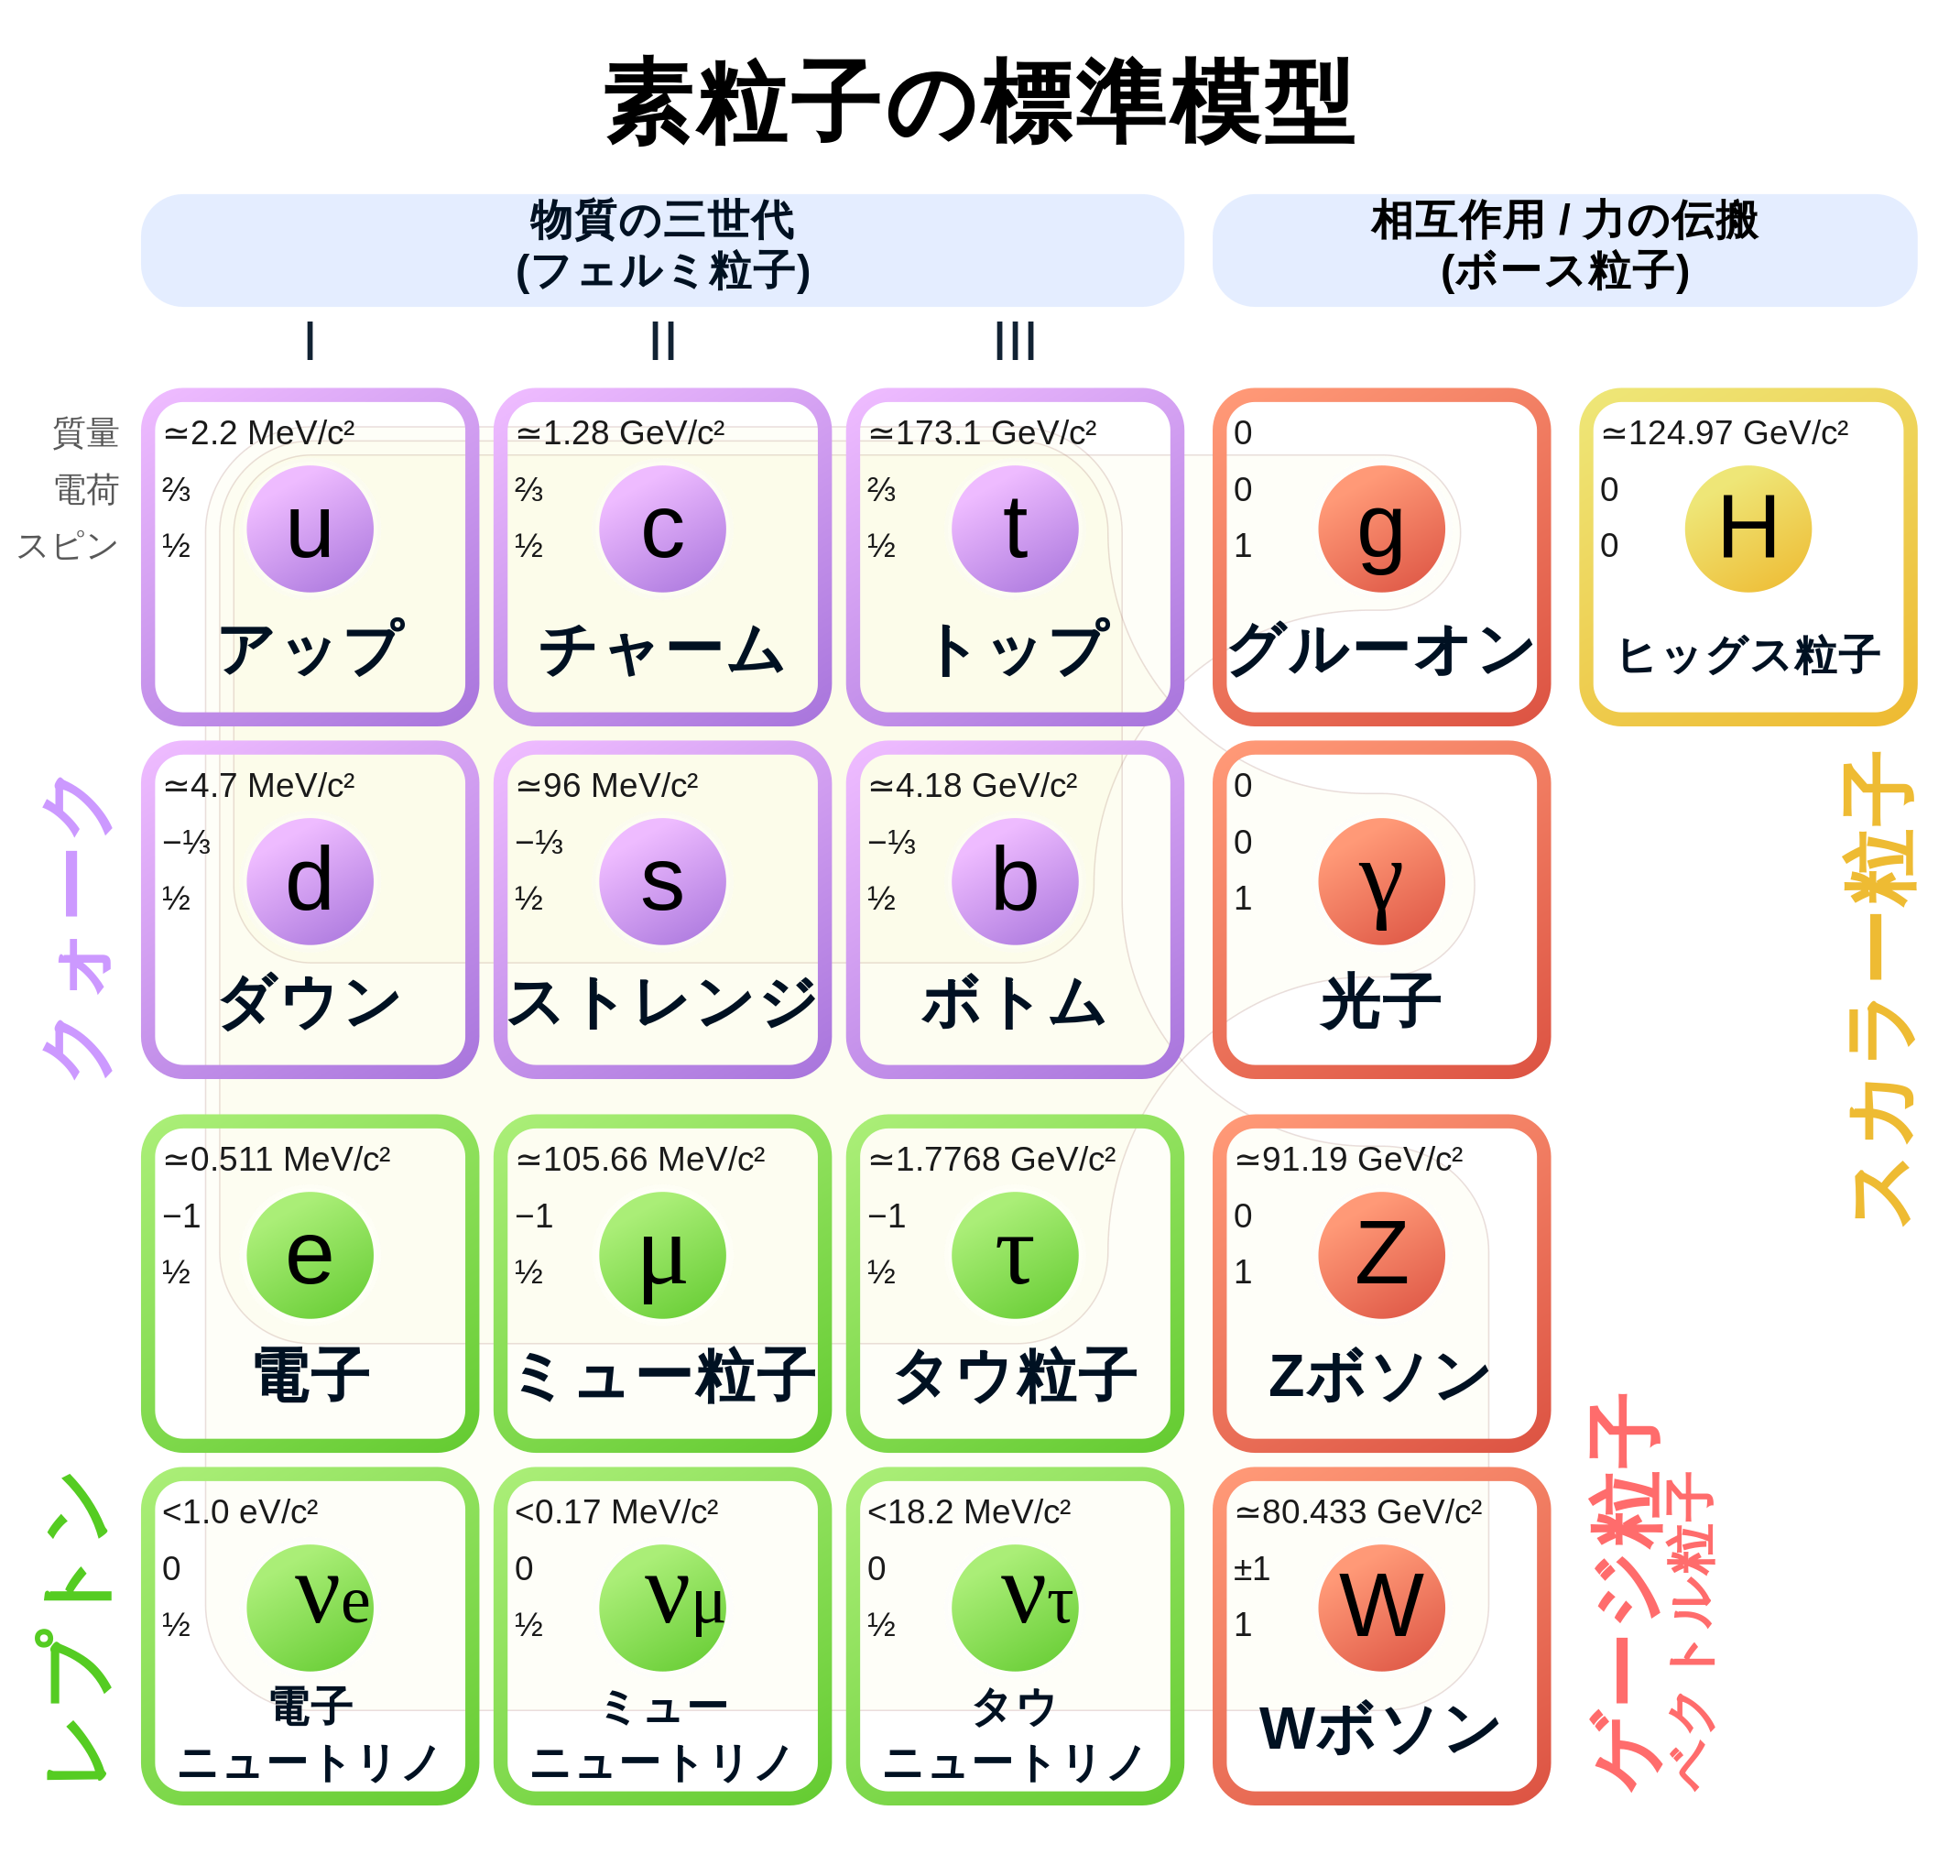
\includegraphics[width=0.38\textwidth]{fig/SM.png}       

      \vspace*{-10pt}
      { \small
        \hspace*{4cm}
        [\href{https://ja.wikipedia.org/wiki/標準模型}{Wikipedia}]
      }   
    \end{center}
  }

  \only<2>{
  \vspace*{10pt}

  標準模型では説明することができない現象がある。
  \begin{itemize}
    \item 
    重力の相互作用
    \item 
    ダークマターなどの未知の粒子
  \end{itemize}

  ([\href{https://www2.yukawa.kyoto-u.ac.jp/~soken.editorial/sokendenshi/vol33/1/修士論文_素粒子研究_内田.pdf}{内田20}]が参考になります。)
  }
  
\end{frame}

\begin{frame}

  これらの問題点を解決する模型として\textcolor{DarkBlue}{高次元時空モデル}が提案される。

  今回の研究では、特に
  \begin{center}
    10次元
    $=$
    \textcolor{DarkRed}{\uwave{\textcolor{black}{4次元ミンコフスキー時空}}}
    $+$
    \textcolor{DarkGreen}{\uwave{\textcolor{black}{6次元余剰空間}}}
  \end{center}
  を考える。  

  \pause

  \begin{tikzpicture}[remember picture, overlay]
    \draw [-latex,DarkRed] (3.0,-0.3)--(6.7,1.2);
    \node at (3.0,-0.3) [below,DarkRed] {私たちから見える時空$x^{0},x^{1},x^{2},x^{3}$};
    \draw [-latex,DarkGreen] (10.0,-0.3)--(10.1,1.2);
    \node at (10.0,-0.3) [below,DarkGreen] {見えないほど小さな空間$y^{4},\cdots,y^{9}$};
    \node at (10.0,-0.9) [below,DarkGreen] {(コンパクト空間)};
  \end{tikzpicture}

\end{frame}

\begin{frame}

  理論は\textcolor{DarkRed}{作用$S$}によって決定される。

  \uline{4次元の場合}\ (e.g.\ スカラー場)
  \begin{equation}
    S
    =
    \int\dd^4 x\ \mathcal{L}
    =
    \int\dd^4 x\ 
    \left(  
      \frac{1}{2}(\partial_{\mu}\phi)(\partial^{\mu}\phi)
      +
      \frac{1}{2}m^2\phi^2
      +
      \frac{\lambda}{4!}\phi^4
    \right)
    \nonumber
  \end{equation}
  \begin{center}
    $m$は質量、$\lambda$は結合定数(粒子の相互作用の強さ)
  \end{center}

  \pause

  \uline{10次元の場合}
  \begin{align}
    S
    &=
    \int\dd^4 x\ \dd^6 y\ 
    \left(  
      \frac{1}{2}(\partial_{\mu}\phi)(\partial^{\mu}\phi)
      +
      \frac{1}{2}\textcolor{DarkOrange}{m^2}\phi(x,y)^2
      +
      \frac{\textcolor{DarkMagenta}{\lambda}}{4!}\phi(x,y)^4
    \right)
    \nonumber
    \\    
    &\xrightarrow{\ y\text{方向で積分}\ }
    \int\dd^4 x\ 
    \left(  
      \frac{1}{2}(\partial_{\mu}\phi)(\partial^{\mu}\phi)
      +
      \frac{1}{2}\textcolor{DarkOrange}{M^2}\phi(x)^2
      +
      \frac{\textcolor{DarkMagenta}{\Lambda}}{4!}\phi(x)^4
    \right)    
    \nonumber
  \end{align}

  \pause

  \begin{bluebox}{\empty}
    \centering
    4次元の$\textcolor{DarkOrange}{M}$や$\textcolor{DarkMagenta}{\Lambda}$の値が余剰空間の幾何(大きさ、形など)で決定される。
  \end{bluebox}

\end{frame}


\begin{frame}

  余剰空間の幾何は力学的な場である計量$\textcolor{NavyBlue}{g_{MN}(x,y)}$によって決定される。
  \begin{equation}
    \dd s^2
    =
    \textcolor{NavyBlue}{g_{\mu\nu}(x,y)} \dd x^{\mu}\dd x^{\nu}
    +
    \textcolor{NavyBlue}{g_{mn}(x,y)} \dd y^{m}\dd y^{n}
    \nonumber
  \end{equation}
  \begin{center}
    余剰空間の計量$\textcolor{NavyBlue}{g_{mn}(x,y)}$を\textcolor{FireBrick}{モジュライ}という。    
  \end{center}

  \pause

  現実の余剰空間の幾何は真空期待値$\textcolor{NavyBlue}{\ev*{g_{mn}}}$に固定されていると考えられる。

  真空期待値$\textcolor{NavyBlue}{\ev*{g_{mn}}}$はそのポテンシャルによって決定される。(\textcolor{FireBrick}{モジュライ固定})
  
  \begin{center}
    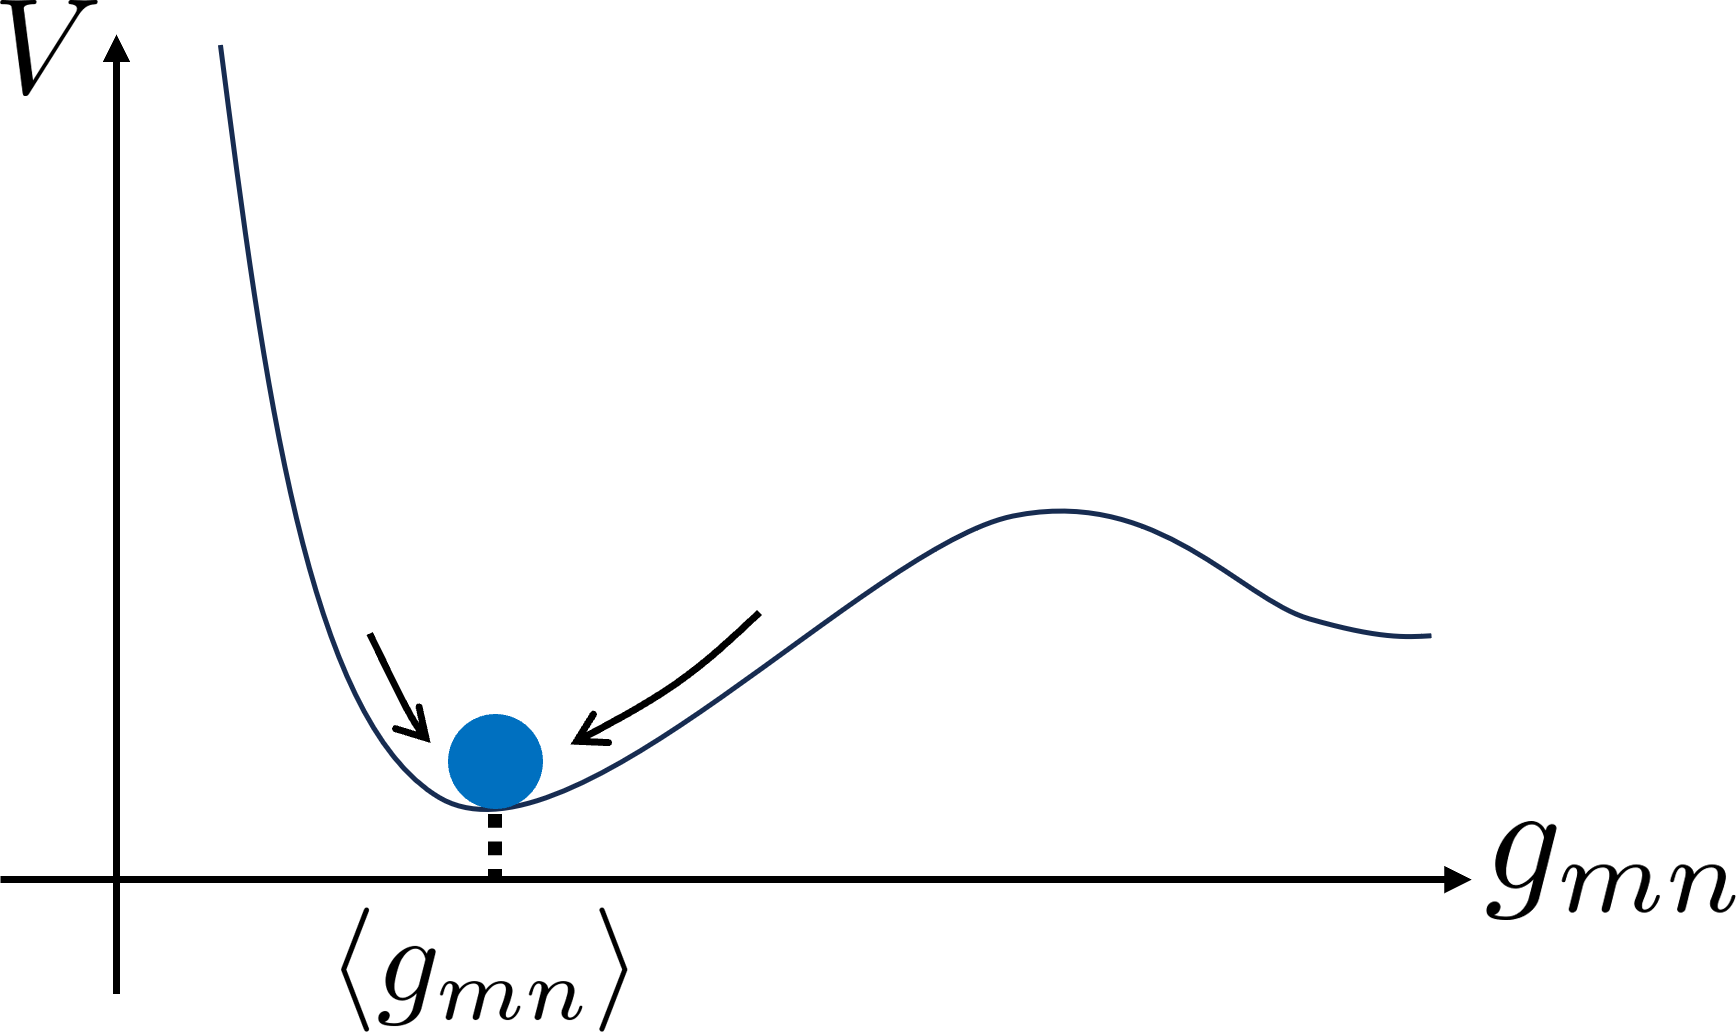
\includegraphics[width=0.5\textwidth]{fig/vev_idea.png}
  \end{center}  

\end{frame}


\begin{frame}

  \begin{bluebox}{本研究の目的}
    \centering
    \begin{itemize}
      \item 
      標準模型を部分的に再現している先行研究[\href{http://arxiv.org/abs/1204.5327}{AKOS12}]のモジュライ固定を議論。
      \item 
      そのモデルから分かる余剰空間の幾何が実際に観測と矛盾ないかを議論。
    \end{itemize}
  \end{bluebox}

\end{frame}


\section{研究内容}

\begin{frame}
  \huge \secname
\end{frame}

\begin{frame}
  
  \uline{磁化トーラス模型}
  \vskip\baselineskip

  6次元余剰空間を\uwave{3つのトーラス$T^{2}$}にコンパクト化。
  \\
  \vspace*{5pt}
  \hspace*{2.8cm}
\includegraphics[width=0.4\textwidth]{fig/tori.png}
  \\
  \hspace*{3.0cm}
  $\mathcal{A}^{(1)}$
  \hspace*{1.0cm}
  $\mathcal{A}^{(2)}$
  \hspace*{1.0cm}
  $\mathcal{A}^{(3)}$
  \hspace*{0.5cm}
  :トーラスの面積(\textcolor{FireBrick}{モジュライ})

  \pause

  \vspace*{1cm}

  \begin{columns}[t]    
    \begin{column}{0.5\textwidth} 
      さらに、トーラス上の2種のゲージ場にそれぞれ磁場$M_{a}^{(i)}$を導入$(a=1,2)$      
    \end{column}
    \begin{column}{0.48\textwidth} 
      \vspace*{-1cm}
      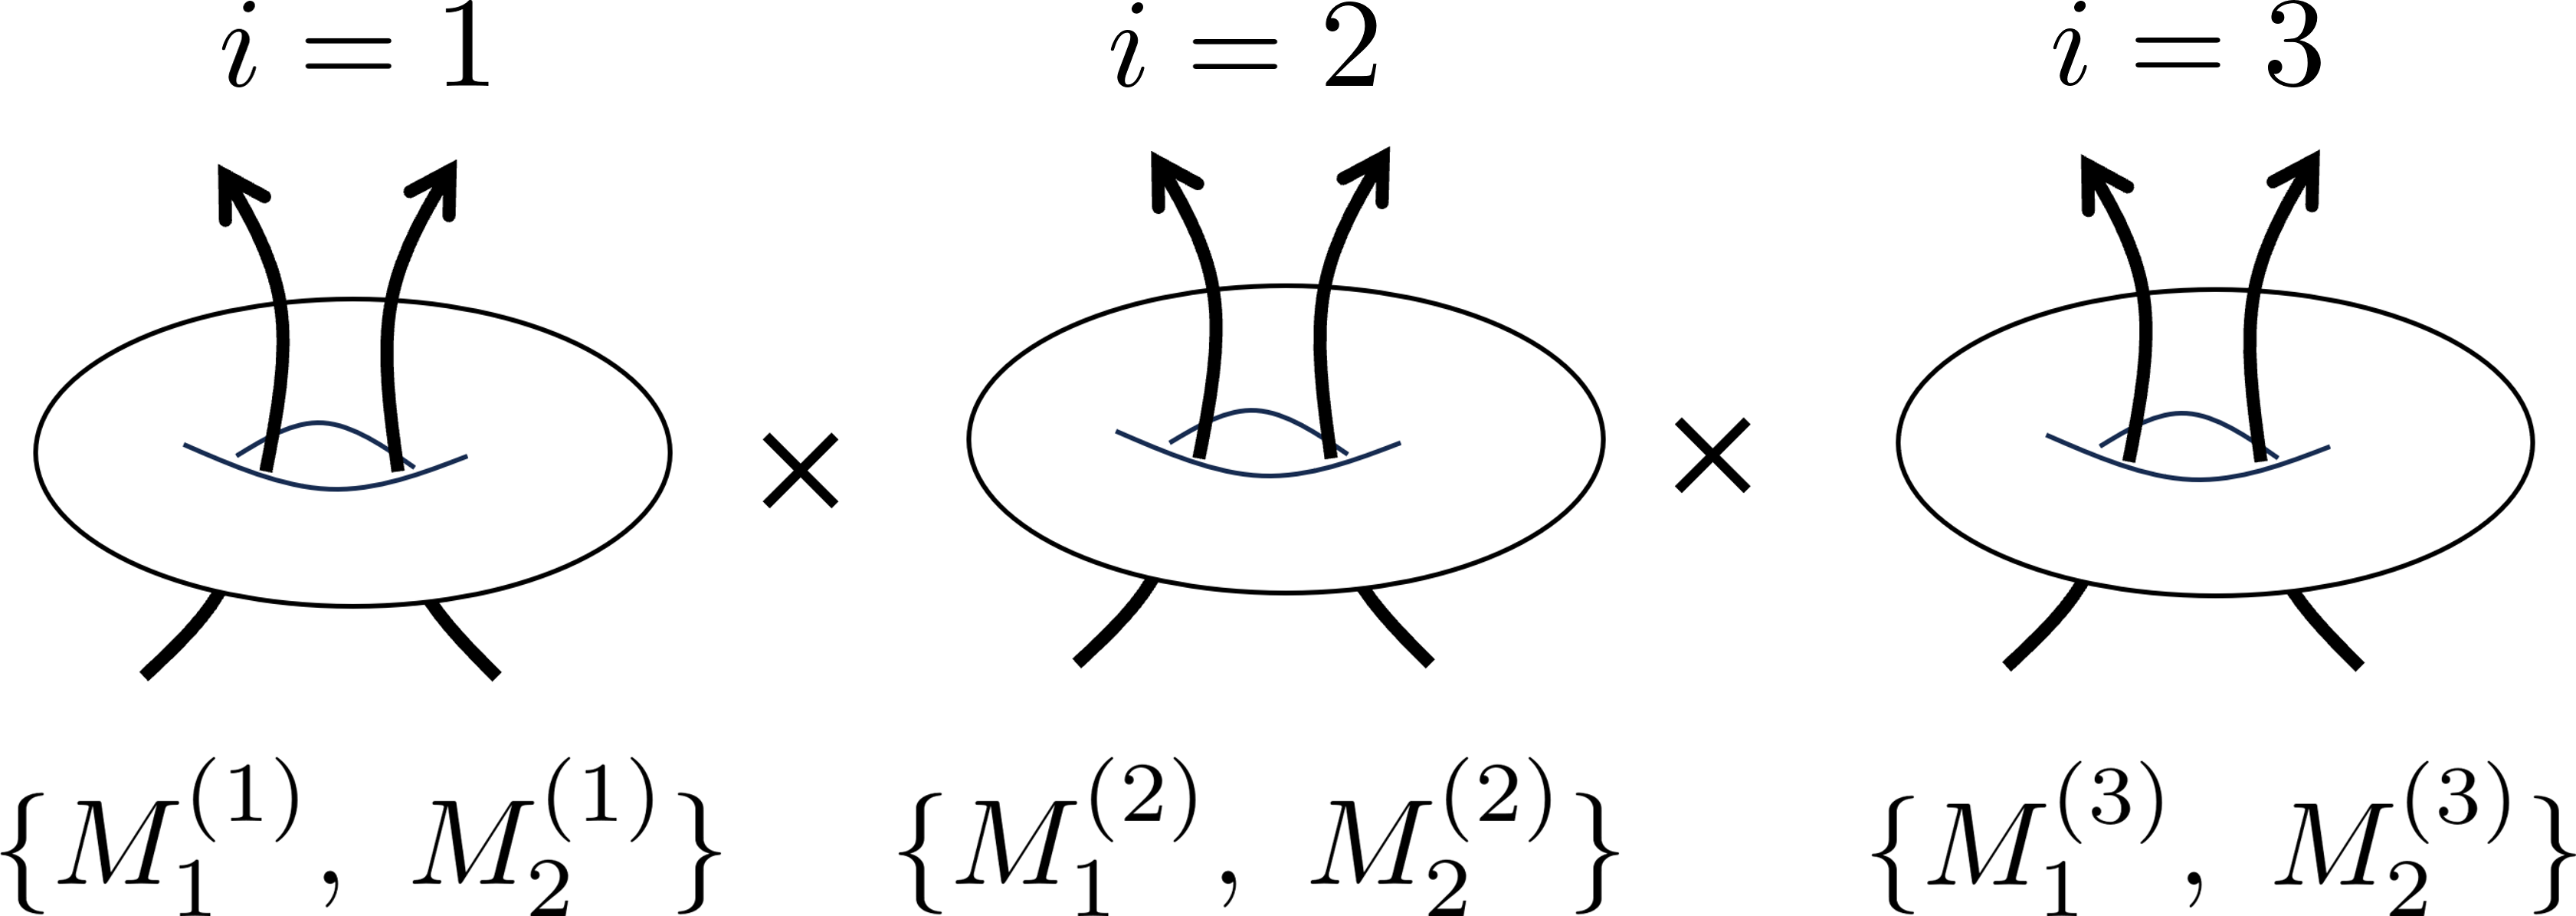
\includegraphics[width=1.0\textwidth]{fig/tori_fluxed.png}
    \end{column}
  \end{columns}

\end{frame}

\begin{frame}
  
  \uline{磁場のポテンシャル}\qquad 
  $
    F^{MN}F_{MN}
    =
    F^{\mu\nu}F_{\mu\nu}
    +
    \uwave{F^{mn}F_{mn}}
    +
    \cdots
  $
  \\
  \hspace*{9cm}{\Large $\downarrow$}
  \begin{equation}
    V^{(D)}
    =
    \pi^2
    \prod_{i}\mathcal{A}^{i}
    \times
    \left\{
      \uline{
      \left(  
        \sum_{i}\frac{M_{1}^{(i)}}{\mathcal{A}^{(i)}}
      \right)^2
      }
      +
      \uline{
      \left( 
        \sum_{i}\frac{M_{2}^{(i)}}{\mathcal{A}^{(i)}}
      \right)^2
      }
    \right\}
    \nonumber
  \end{equation}
  \hspace*{6.2cm}
  それぞれがゼロのときに$\ev*{V^{(D)}}=0$\ (最小)

  \begin{center}
    \tikz[baseline=(x.base)]{
      \node(x)[rectangle, fill=DarkRed!10, rounded corners]{
        \ 
        $
        \displaystyle
        \frac{M_{a}^{(1)}}{\ev*{\mathcal{A}^{(1)}}}
        +
        \frac{M_{a}^{(2)}}{\ev*{\mathcal{A}^{(2)}}}
        +
        \frac{M_{a}^{(3)}}{\ev*{\mathcal{A}^{(3)}}}
        =
        0
        \quad
        \text{for}
        \ 
        a=1,2$\ };
    }    
  \end{center}

\end{frame}

\begin{frame}
  
  \uline{真空期待値$\ev*{\mathcal{A}^{(1)}},\ev*{\mathcal{A}^{(2)}},\ev*{\mathcal{A}^{(3)}}$の関係}
  \begin{gather}
    M_{a}^{(1)}
    +
    M_{a}^{(2)}
    \frac{\ev*{\mathcal{A}^{(1)}}}{\ev*{\mathcal{A}^{(2)}}}
    +
    M_{a}^{(3)}
    \frac{\ev*{\mathcal{A}^{(1)}}}{\ev*{\mathcal{A}^{(3)}}}
    =
    0
    \quad
    \text{for}
    \ 
    a=1,2
    \nonumber    
    \\
    \text{\Large $\downarrow$}
    \nonumber
    \\
    \hspace*{-10pt}
    \frac{\ev*{\mathcal{A}^{(1)}}}{\ev*{\mathcal{A}^{(2)}}}
    =
    \frac{
      M_{1}^{(3)} M_{2}^{(1)}-M_{1}^{(1)} M_{2}^{(3)}
    }{
      M_{1}^{(2)} M_{2}^{(3)}- M_{1}^{(3)} M_{2}^{(2)}
    }
    \ ,\ 
    \frac{\ev*{\mathcal{A}^{(1)}}}{\ev*{\mathcal{A}^{(3)}}}
    =
    -\frac{
      M_{1}^{(2)} M_{2}^{(1)}-M_{1}^{(1)} M_{2}^{(2)}
    }{
      M_{1}^{(2)} M_{2}^{(3)}-M_{1}^{(3)} M_{2}^{(2)}
    }
    \nonumber
  \end{gather}
  \begin{redbox}{\empty}
    \centering
    面積の比は磁場のポテンシャルによって決定された。
  \end{redbox}
  
\end{frame}

\begin{frame}
  
  余剰空間に磁場を導入すると、\textcolor{DarkRed}{トーラスの面積比が決定}された。
  \vskip\baselineskip

  \pause

  ただし、面積の値を決定するためには\textcolor{DarkGreen}{全体の因子}がまだ不定。
  \vskip\baselineskip

  \pause

  \begin{bluebox}{今後の方針}
    \centering
    磁場とは異なる起源をもつポテンシャルを導入して\\
    \textcolor{DarkGreen}{全体の因子}を決定する\textcolor{FireBrick}{モジュライ}を固定
  \end{bluebox}

\end{frame}

\begin{frame}  

  全体の因子を決定するモジュライ:$T\quad (\propto\ev*{\mathcal{A}^{(1)}},\ev*{\mathcal{A}^{(2)}},\ev*{\mathcal{A}^{(3)}})$
  \vskip\baselineskip

  \uline{$T$の有効ポテンシャル}
  \begin{itemize}
    \item 
    有効理論は超対称性(ボゾンとフェルミオンの対称性)をもつ
    \item
    超対称作用はスーパーポテンシャル$W$とケーラーポテンシャル$K$で決定
    \item
    本研究では以下のポテンシャルを用いる[\href{http://arxiv.org/abs/hep-th/0611024}{AHKO07}]:
    \begin{equation}
      \left\{
        \begin{alignedat}{1}
          W
          &=
          w_{0}-Ae^{-a\textcolor{DarkRed}{T}}+B\textcolor{DarkBlue}{X}
          \\
          K
          &=
          -
          \ln (\textcolor{DarkRed}{T}+\textcolor{DarkRed}{\bar{T}})
          +
          \textcolor{DarkBlue}{|X|^2}
        \end{alignedat}
      \right.
      \nonumber
    \end{equation}
    \begin{center}
      \small
      $\textcolor{DarkBlue}{X}$は新たに導入したスカラー場
      ,
      $w_{0}, A, B, a$は実パラメター      
    \end{center}
  \end{itemize}

\end{frame}

\begin{frame}

  \vspace*{1.2cm}

  プランクスケール$M_{\text{Pl}}(\sim 2.4\times 10^{18}\ \text{GeV})=1$の単位系

  \begin{columns}[t]    
    \begin{column}{0.6\textwidth} 
      \uline{スカラーポテンシャル}
      \vspace*{-5pt}
      \begin{gather}
        V^{(F)}
        =
        e^{K}(K^{I\bar{J}}(D_{I}W)(D_{\bar{J}}\bar{W})-3|W|^2)
        \nonumber
        \\
        \left\{
          \begin{alignedat}{1}
            D_{I}W
            &\equiv
            \partial_{I}W+(\partial_{I}K)W
            \\
            K^{I\bar{J}}
            &\text{:$\partial_{I}\partial_{\bar{J}}K$の逆行列}        
          \end{alignedat}
        \right.
        \quad
        (I=X,T)
        \nonumber
      \end{gather}
    \end{column}
    \begin{column}{0.38\textwidth} 
      \vspace*{-5pt}
      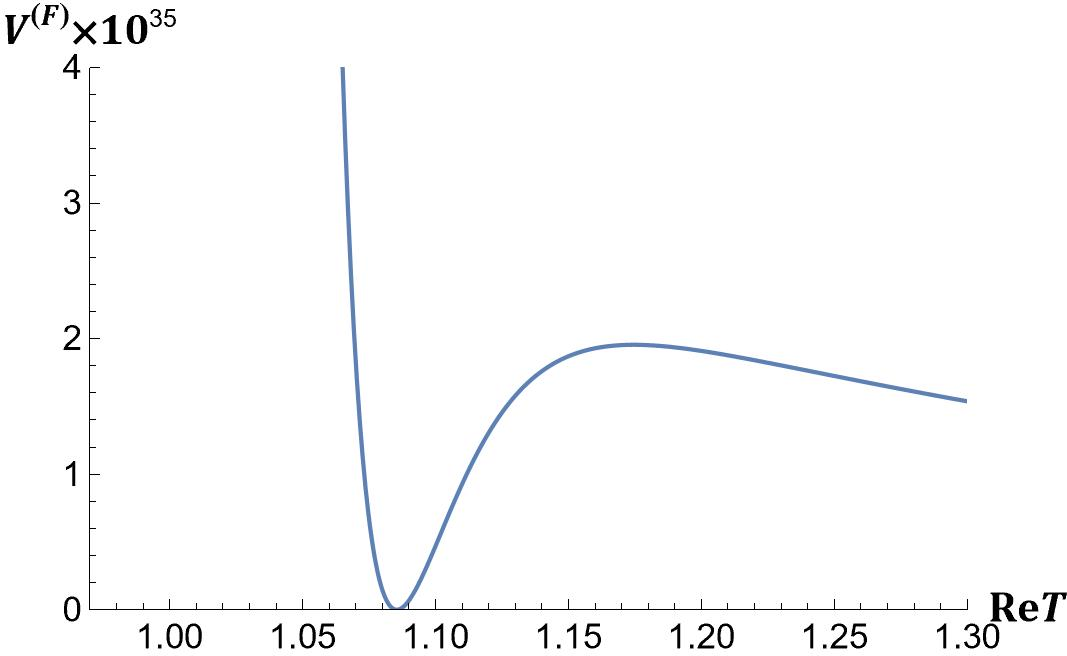
\includegraphics[width=1.0\textwidth]{fig/result.jpg}
    \end{column}
  \end{columns}

  \vspace*{10pt}

  パラメター:
    $
    w_{0}
    \sim
    2.17
    \times
    10^{-18}
    \ ,\ 
    a=4\pi^2
    \ ,\ 
    A=1
    \ ,\ 
    B=e^{-4\pi^2}
    $
  \begin{center}
    $\rightarrow \ev*{T}\sim 1.085$に固定
  \end{center}

  \begin{tikzpicture}[remember picture, overlay]
    \node[anchor=north east, align=left] at ($(current page.north east)-(0,0.7)$){
    {      
      \small
      \tikz[baseline=(x.base)]{
        \node(x)[rectangle, fill=blue!10, rounded corners]{
          $W
          =
          w_{0}-Ae^{-a\textcolor{DarkRed}{T}}+B\textcolor{DarkBlue}{X}
          \ ,\ 
          K
          =
          -
          \ln (\textcolor{DarkRed}{T}+\textcolor{DarkRed}{\bar{T}})
          +
          \textcolor{DarkBlue}{|X|^2}$};
      }
    }
    };
  \end{tikzpicture}

\end{frame}

\begin{frame}

  磁場の値は先行研究[\href{http://arxiv.org/abs/1703.03402}{AKSU17}]の値:標準模型の世代構造を再現
  \begin{center}
    \small
    $
      \{M_{1}^{(1)},M_{2}^{(1)}\}
      =
      \{7,-7\}
      \ ,\ 
      \{M_{1}^{(2)},M_{2}^{(2)}\}
      =
      \{1,0\}
      \ ,\ 
      \{M_{1}^{(3)},M_{2}^{(3)}\}
      =
      \{0,-1\}        
    $
  \end{center}

  \begin{center}      
    面積比\quad
    \tikz[baseline=(x.base)]{
      \node(x)[rectangle, fill=DarkRed!10, rounded corners]{
        \        
    $\displaystyle
    \frac{\mathcal{A}^{(2)}}{\mathcal{A}^{(1)}}
    =
    \frac{\mathcal{A}^{(3)}}{\mathcal{A}^{(1)}}
    =
    \frac{1}{7}    
    $\ };
    }    
    \qquad\quad
    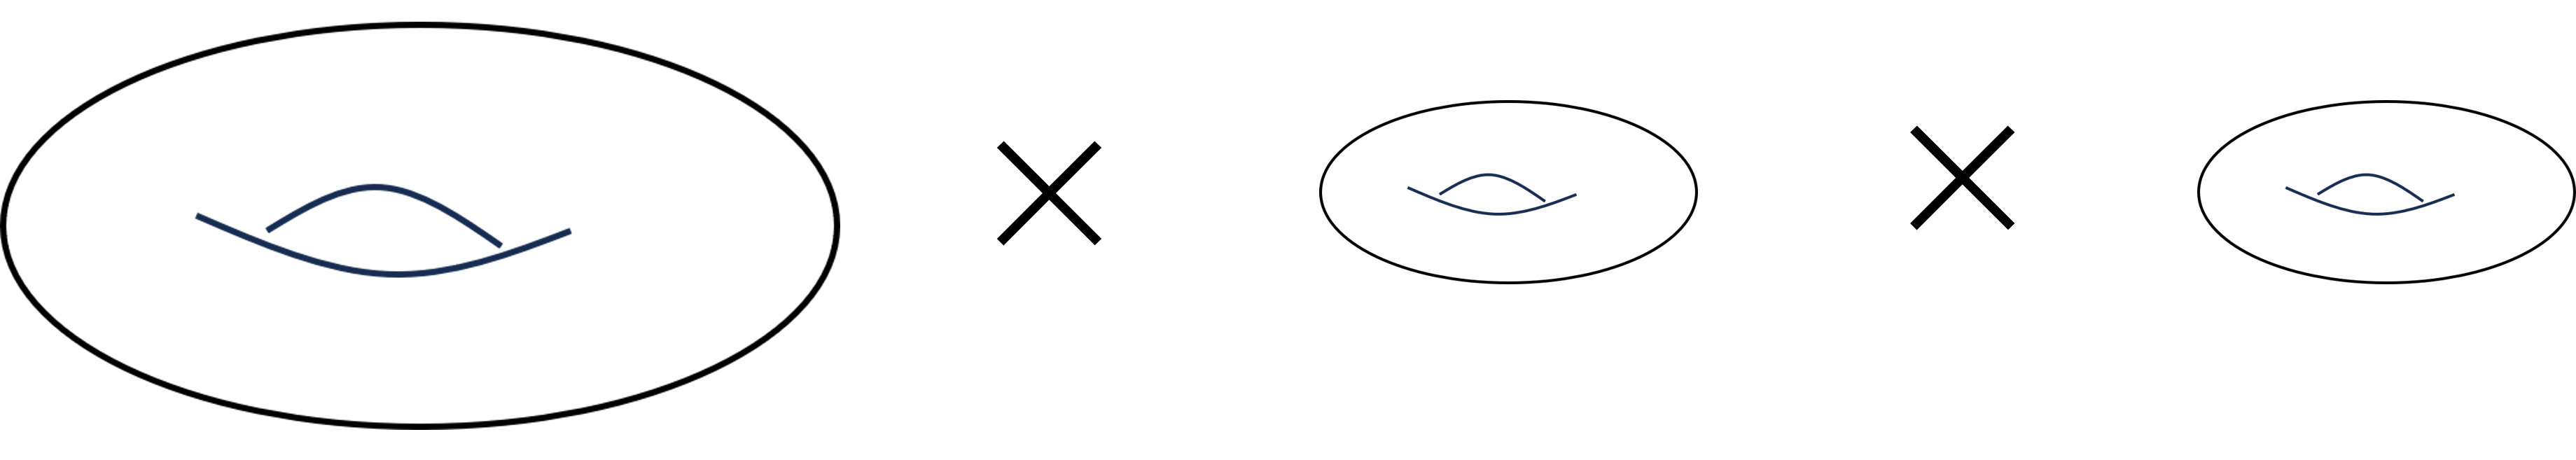
\includegraphics[width=0.55\textwidth]{fig/result_ori.png}
  \end{center}

  \vspace*{-10pt}
  \pause

  \begin{center}
    \hspace*{-24pt}
    \begin{tabular}{rl|c}
      & 
      第1トーラスの面積 & 実験による制限([\href{https://pdg.lbl.gov/2023/tables/rpp2023-sum-searches.pdf}{PDG}]) \\
      $\ev*{\mathcal{A}^{(1)}}$ & $\sim (10^{-35}\ \text{m})^2$ & $R_{6\text{D}}<\mathcal{O}(10^{-6}\ \text{m})$
      \\
      & $\sim (10^{19}\ \text{GeV})^{-2}$ & $M_{\text{KK}}>\mathcal{O}(10^{3}\ \text{GeV})$
    \end{tabular}
  \end{center}

\end{frame}


\section{まとめ・展望}

\begin{frame}

  \uline{まとめ}
  \begin{itemize}
    \item 
    磁化トーラス模型におけるモジュライ(トーラスの面積)の固定を議論
    \item 
    面積比は磁場のポテンシャル$V^{(D)}$のみで決定(ただし、全体の因子は不定)
    \item 
    磁場とは異なる起源をもつポテンシャル$V^{(F)}$により全体の因子を決定
  \end{itemize}

  \uline{展望}
  \begin{itemize}
    \item 
    より一般的なポテンシャル$V^{(F)}$によるモジュライ固定
    \item 
    超対称性の自発的破れ、超対称粒子の質量などについて議論
  \end{itemize}
  
\end{frame}


% --------------------------

% \newcounter{Appendix}
% \setcounter{Appendix}{\value{framenumber}}
% \setcounter{section}{0}
% \renewcommand{\thesubsection}{\Alph{subsection}}
% \makeatletter
%    \renewcommand{\theequation}{\thesubsection.\arabic{equation}}
%    \@addtoreset{equation}{section}
   
%    \renewcommand{\thefigure}{\thesubsection.\arabic{figure}}
%    \@addtoreset{figure}{section}
   
%    \renewcommand{\thetable}{\thesubsection.\arabic{table}}
%    \@addtoreset{table}{section}
% \makeatother

% \section{付録}

% \begin{frame}[plain]
%   \frametitle{\ }
%   \huge \secname
% \end{frame}

% \begin{frame}[plain]
%   \frametitle{\thesubsection\ \subsecname}







  
% \end{frame}

% --------------------------

% \section{参考文献}
% \begin{frame}[plain,allowframebreaks]
%   \frametitle{\secname}
%   \scriptsize
%   \beamertemplatetextbibitems
%   \bibliography{ref}
%   \bibliographystyle{unsrt}

%   \nocite{Wess:1992}

% \end{frame}


% \setcounter{framenumber}{\value{Appendix}}
\end{document}
